\chapter{Comparing the effects of different lifting operators and Investigating Numerical Stability in Fluid-Structure Interaction problems}\label{sec:mesh_motion}
The first section is devoted to comparing different lifting operators defined in section \ref{sec:meshmotion}. The choice of lifting operators is crucial when computing FSI problems. When handling large structural deformations one has to be very cautious about the choice of lifting operators. A good lifting operator upholds the integrity of the computational domain, allowing large deformations in the solid and into the fluid domain. The computational cost is different of the different lifting operators, and it is therefore crucial to chose the right lifting operator for a specific problem. 

The second section investigates briefly the impact of choosing different value for $\theta$ in the $\theta$-scheme. The effects of choosing a Crank-Nicholson or a backward Euler scheme is known to have effects on the energy preservation in a computational system. Also the effects of shifting the Crank-Nicholson scheme is investigated using the FSI2 and FSI3 case from the previous chapter.
\section{Methods for comparing lifting operators}
The comparisons will be performed using a version of the CSM1 test as defined the previous chapter, with the same computing domain and parameters. The version of CSM1 test case is now computed as a full FSI problem with the fluid initially at rest. A gravitational force is applied to the structure much like the previous CSM test. The only difference is that we now use the full domain from the \ref{sec:HronTurek}. The test is run as time-dependent with a the backward Euler scheme, leading to a steady state solution.

The tests will compare the different operators by investigating how the deformation from the solid domain is lifted into the fluid domain. I investigate plots of the mesh after deformation to see how much cells distort and where the cells distort. This is visualized using Paraview with its built in function \textit{warp by vector}, which redistributes nodes based on the displacement values in each nodal point.
The computing domain is the same as used in the Hron Turek benchmark, from the previous section.
The upper, lower and left boundary is set as \say{no slip} condition. The left boundary is set to \say{do nothing}, and zero pressure. \newline

The different operators will be plotted with the minimal value of the Jacobian. The Jacobian is also known as the volume ratio, and if the Jacobian is zero anywhere in the domain it means that the volume is negative, and cells overlap. Which can cause singularity in the matrices during assembly. When cells overlap it can in the best case cause the computed numerical code to diverge, and in the worst case just give very wrong results. \newline

A plot of the deformation in the domain has been added, to visualize how the different mesh motion techniques work. It is possible to see that if get thin triangles in the computational domain then the lifting operator is not good enough, and we might get singularities in the computing matrix.
I also looked at how different lifting operators react differently in the FSI2 and FSI3 test cases from the previous section. Here I investigated plots of the lift, drag and displacements too see how the different lifting operators respond to different inflow velocities and solid parameters. Bc1 and bc2 denotes the boundary conditions 1 and 2 used when employing the biharmonic lifting operator.


\subsubsection*{Different lifting operators with testcase CSM1}

Figure \ref{fig:fluid_structure} which shows the minimum of the Jacobian of the entire domain. The harmonic operator with a constant $\alpha_u$ parameter, gives overlapping cells
While the harmonic lifting operator with variable $\alpha_u$ and both the biharmonic techniques, uphold the cells quality.

Figure \ref{fig:CSM1_pictures} shows the meshes of the different lifting operators, for the steady state solutions from the CSM1 test case. The harmonic with a spatial dependent variable $\alpha_u$ and the two biharmonic lifting operators upholds good integrity of the cells. While the harmonic lifting operator with a constant $\alpha_u$ shows degeneration of cells at the tip of the bar. However, the computed numerical code was able to compute with the harmonic constant $\alpha_u$ operator, but as we can see in table \ref{tab:comparing lifting} the displacement values are incorrect.

\begin{figure}[H]
  \label{fig:fluid_structure}
  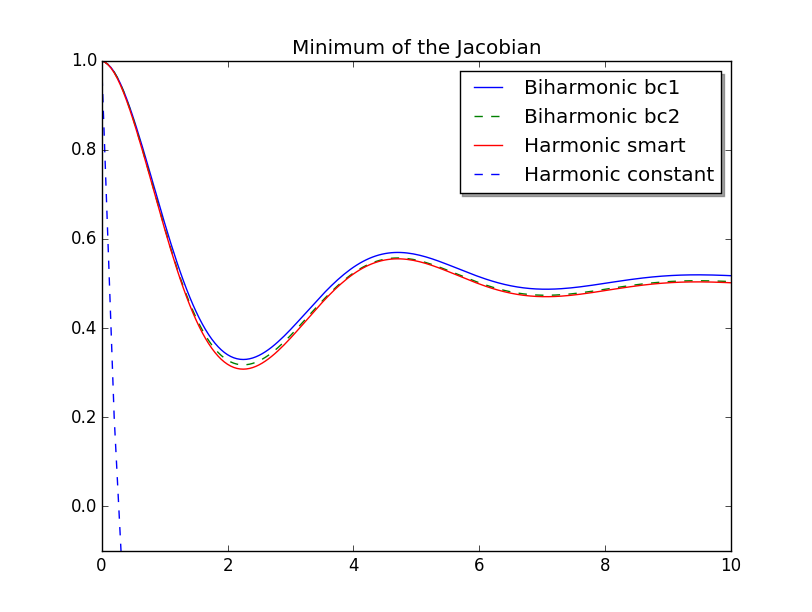
\includegraphics[scale=0.60, trim={0mm 0mm 0mm 0mm},clip]{./Mesh_motion_results/CSM1.png}
   \caption{plot of the minimum of J in entire domain, using CSM1 test. $\Delta t = 0.05$}
\end{figure}

\begin{figure}[H]  
  \begin{minipage}[b]{0.6\linewidth}
    \centering
    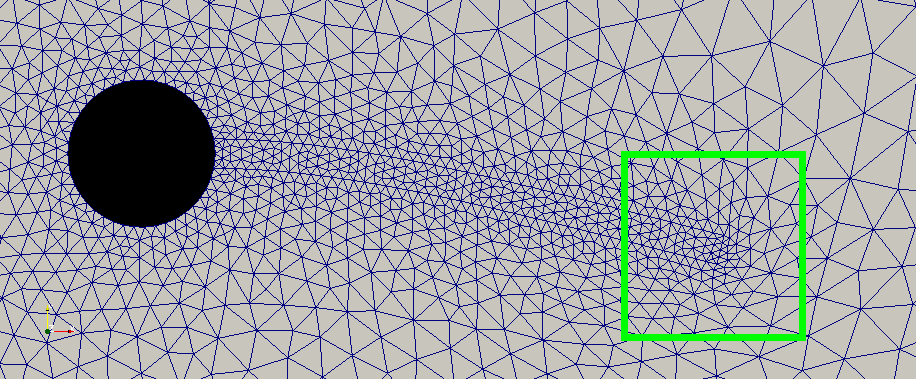
\includegraphics[scale=0.25]{./Mesh_motion_results/CSM1_laplace_rectangle.png} 
    \caption{Harmonic lifting operator with spatial dependent $\alpha_u$} 
    \vspace{4ex}
  \end{minipage}%%
  \begin{minipage}[b]{0.6\linewidth}
    \centering
    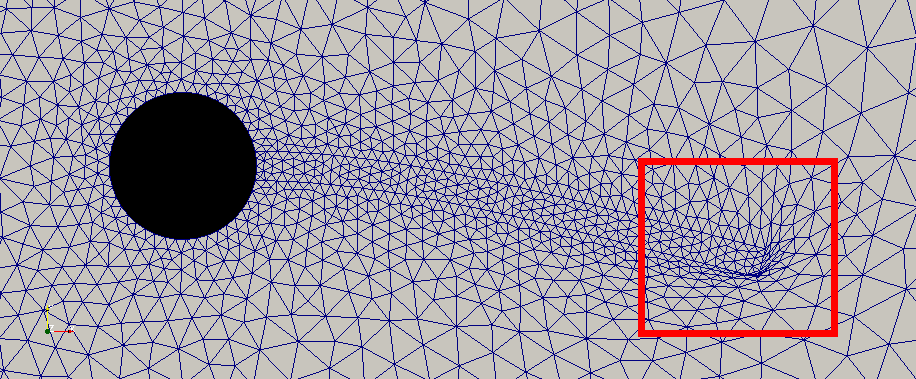
\includegraphics[scale=0.25]{./Mesh_motion_results/CSM1_constant_rectangle.png} 
    \caption{Harmonic lifting operator with constant $\alpha_u$} 
    \vspace{4ex}
  \end{minipage} 
  \begin{minipage}[b]{0.6\linewidth}
    \centering
    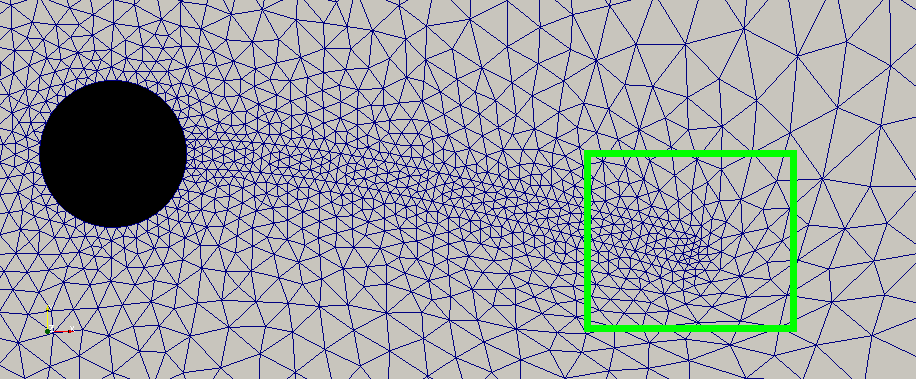
\includegraphics[scale=0.25]{./Mesh_motion_results/CSM1_bibc1_rectangle.png} 
    \caption{Biharmonic lifting operator with boundary condition 1} 
    \vspace{4ex}
  \end{minipage}%% 
  \begin{minipage}[b]{0.6\linewidth}
    \centering
    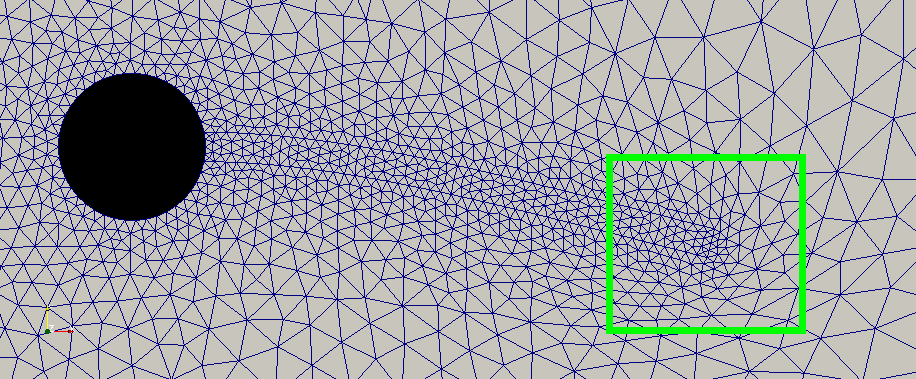
\includegraphics[scale=0.25]{./Mesh_motion_results/CSM1_bibc2_rectangle.png} 
    \caption{Biharmonic lifting operator with boundary conditions 2} 
    \vspace{4ex}
  \end{minipage} 
  \caption{Results of testing different lifting operator using the CSM1 testcase computing full FSI. Green square denoting good cell integrity.}
  \label{fig:CSM1_pictures} 
\end{figure}

\begin{table}[H]
\centering
\caption{Displacements results of different lifting operators of CSM1 test}
\label{tab:comparing lifting}
\begin{tabular}{|l|l|l|}
\hline
Technique & $d_y(A) [\times 10^{-3}]$ & $d_x(A) [\times 10^{-3}]$ \\ \hline
Harmonic & -65.406 & -7.036 \\ \hline
Constant & -43.033 & -2.999 \\ \hline
Bibc1 & -65.404 & -7.036 \\ \hline
Bibc2 & -65.405 & -7.036 \\ \hline
Hron \& Turek & $\bold{-66.10}$& $\bold{-7.187}$\\ \hline
\end{tabular}
\end{table}

\subsubsection{FSI2 with different Lifting operator}

Figure \ref{fig:FSI2_motion-1} shows the harmonic and the two biharmonic mesh motion techniques for the FSI2 case. All three are similar and only a slight change in the period can be noticed.
 
\begin{figure}[H]  
  \begin{minipage}[b]{0.6\linewidth}
    \centering
    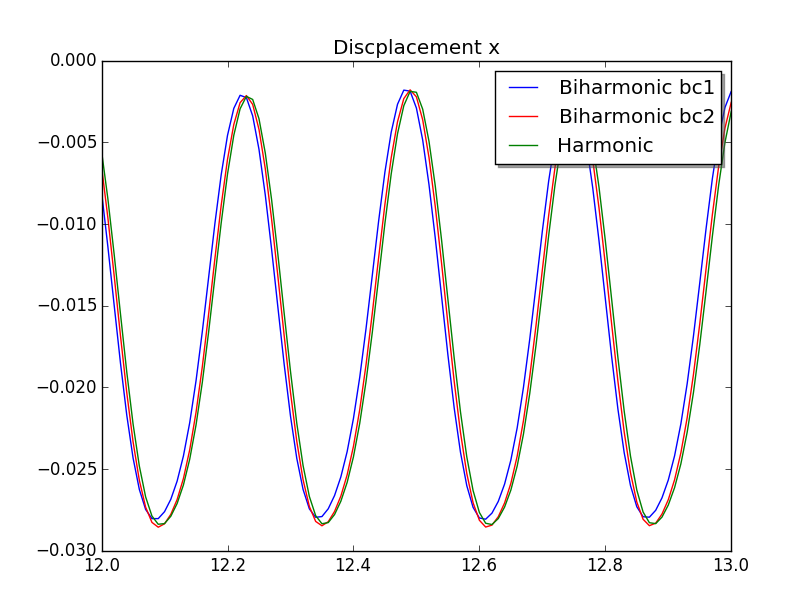
\includegraphics[scale=0.40]{./Mesh_motion_results/FSI2_dt001_dis_x.png} 
    \vspace{4ex}
  \end{minipage}%%
  \begin{minipage}[b]{0.6\linewidth}
    \centering
    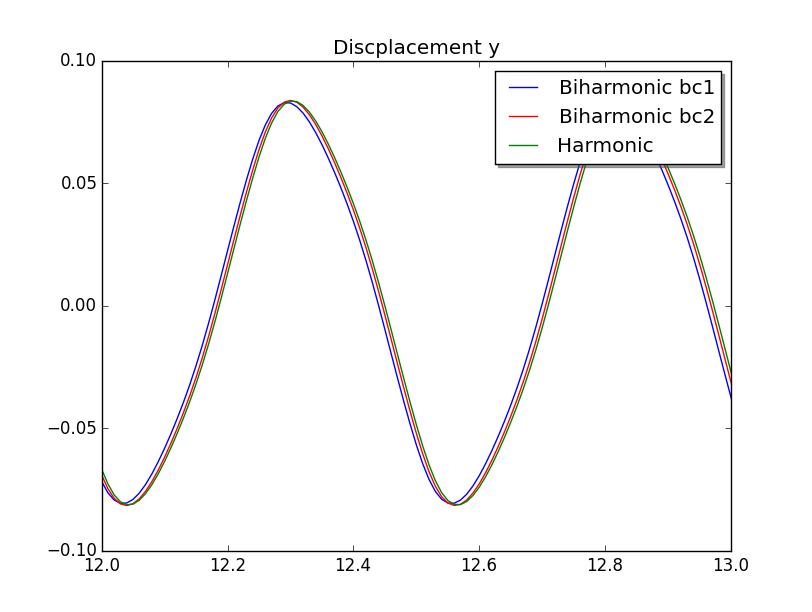
\includegraphics[scale=0.40]{./Mesh_motion_results/FSI2_dt001_dis_y.png} 
    \vspace{4ex}
  \end{minipage} 
  \begin{minipage}[b]{0.6\linewidth}
    \centering
    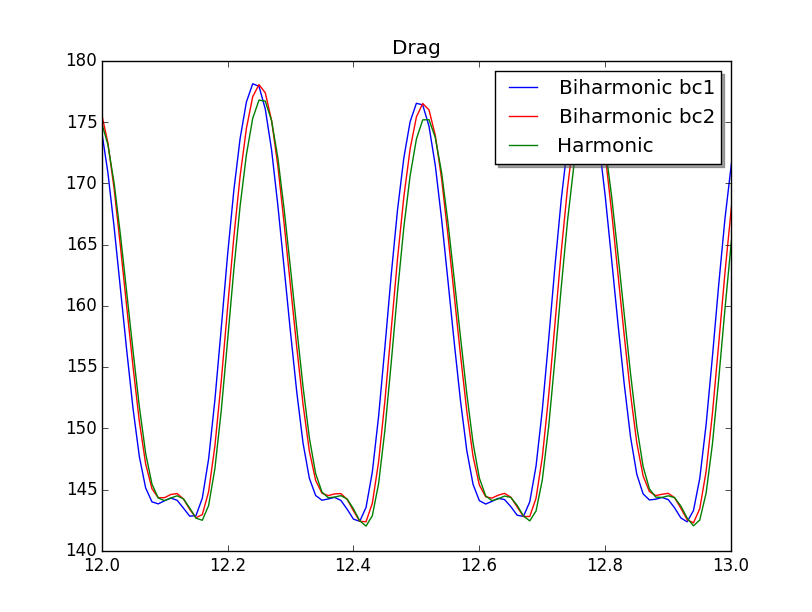
\includegraphics[scale=0.40]{./Mesh_motion_results/FSI2_dt001_drag.png} 
    \vspace{4ex}
  \end{minipage}%% 
  \begin{minipage}[b]{0.6\linewidth}
    \centering
    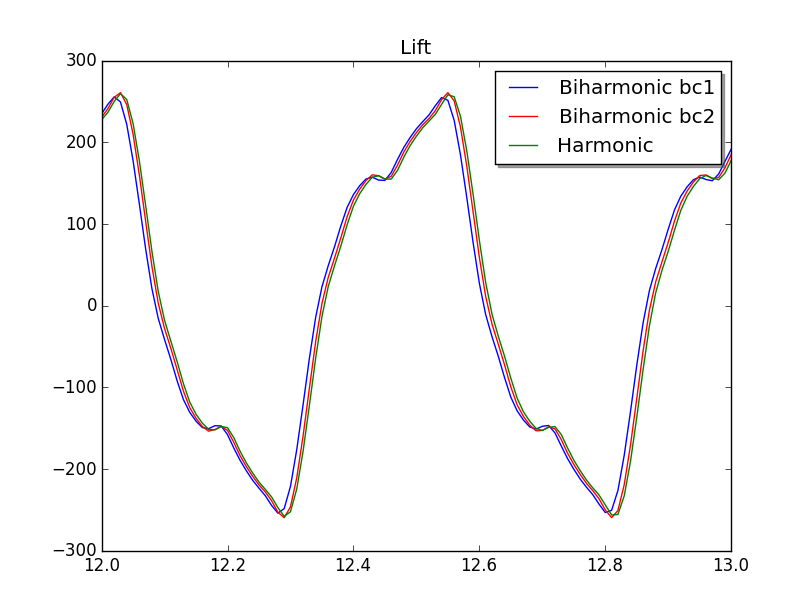
\includegraphics[scale=0.40]{./Mesh_motion_results/FSI2_dt001_lift.png} 
    \vspace{4ex}
  \end{minipage} 
\caption {FSI2 with different lifting operators: harmonic, biharmonic bc1 and bc2. $\Delta t = 0.01$}
\label{fig:FSI2_motion-1} 
\end{figure}

Figure \ref{FSI31}, \ref{FSI32}, \ref{FSI33} and \ref{FSI34} shows the displacement in x and y direction, and drag and lift plots respectively. The displacements and Lift plots show only a slight change in the period. While the Drag for the harmonic lifting operator with mesh dependent $\alpha_u$ shows an increasing in the Drag value of about 10.

\begin{figure}[] 
    \label{FSI31}
    \centering	
    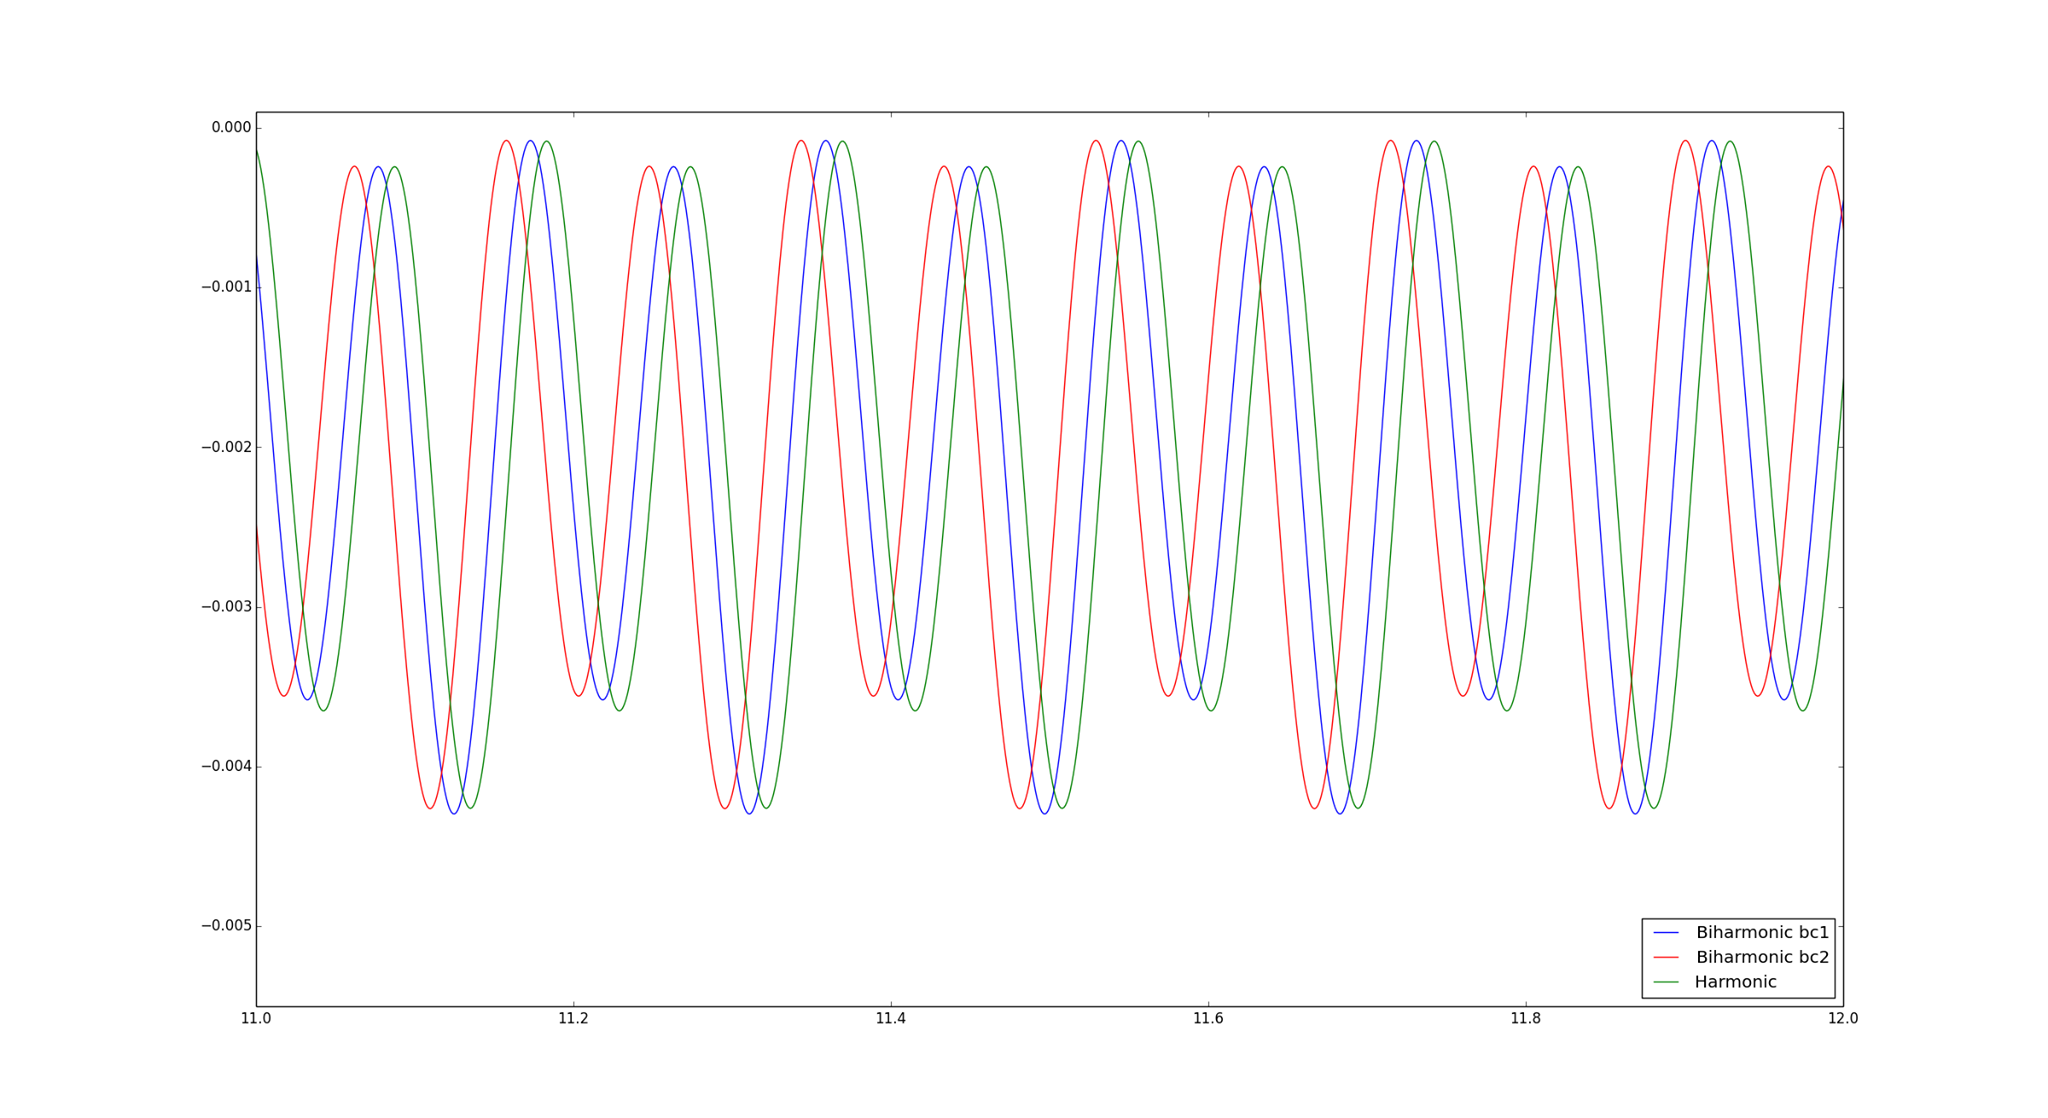
\includegraphics[trim={3cm 3cm 3cm 3cm},clip,scale=0.20]{./Mesh_motion_results/FSI3_dt0001_dis_x.png} 
    \caption{Displacement in x direction for FSI3 with different lifting operators: Harmonic, Biharmonic bc1 and bc2. $\Delta t = 0.001$}
\end{figure}
\begin{figure}[]
    \label{FSI32}
    \centering
    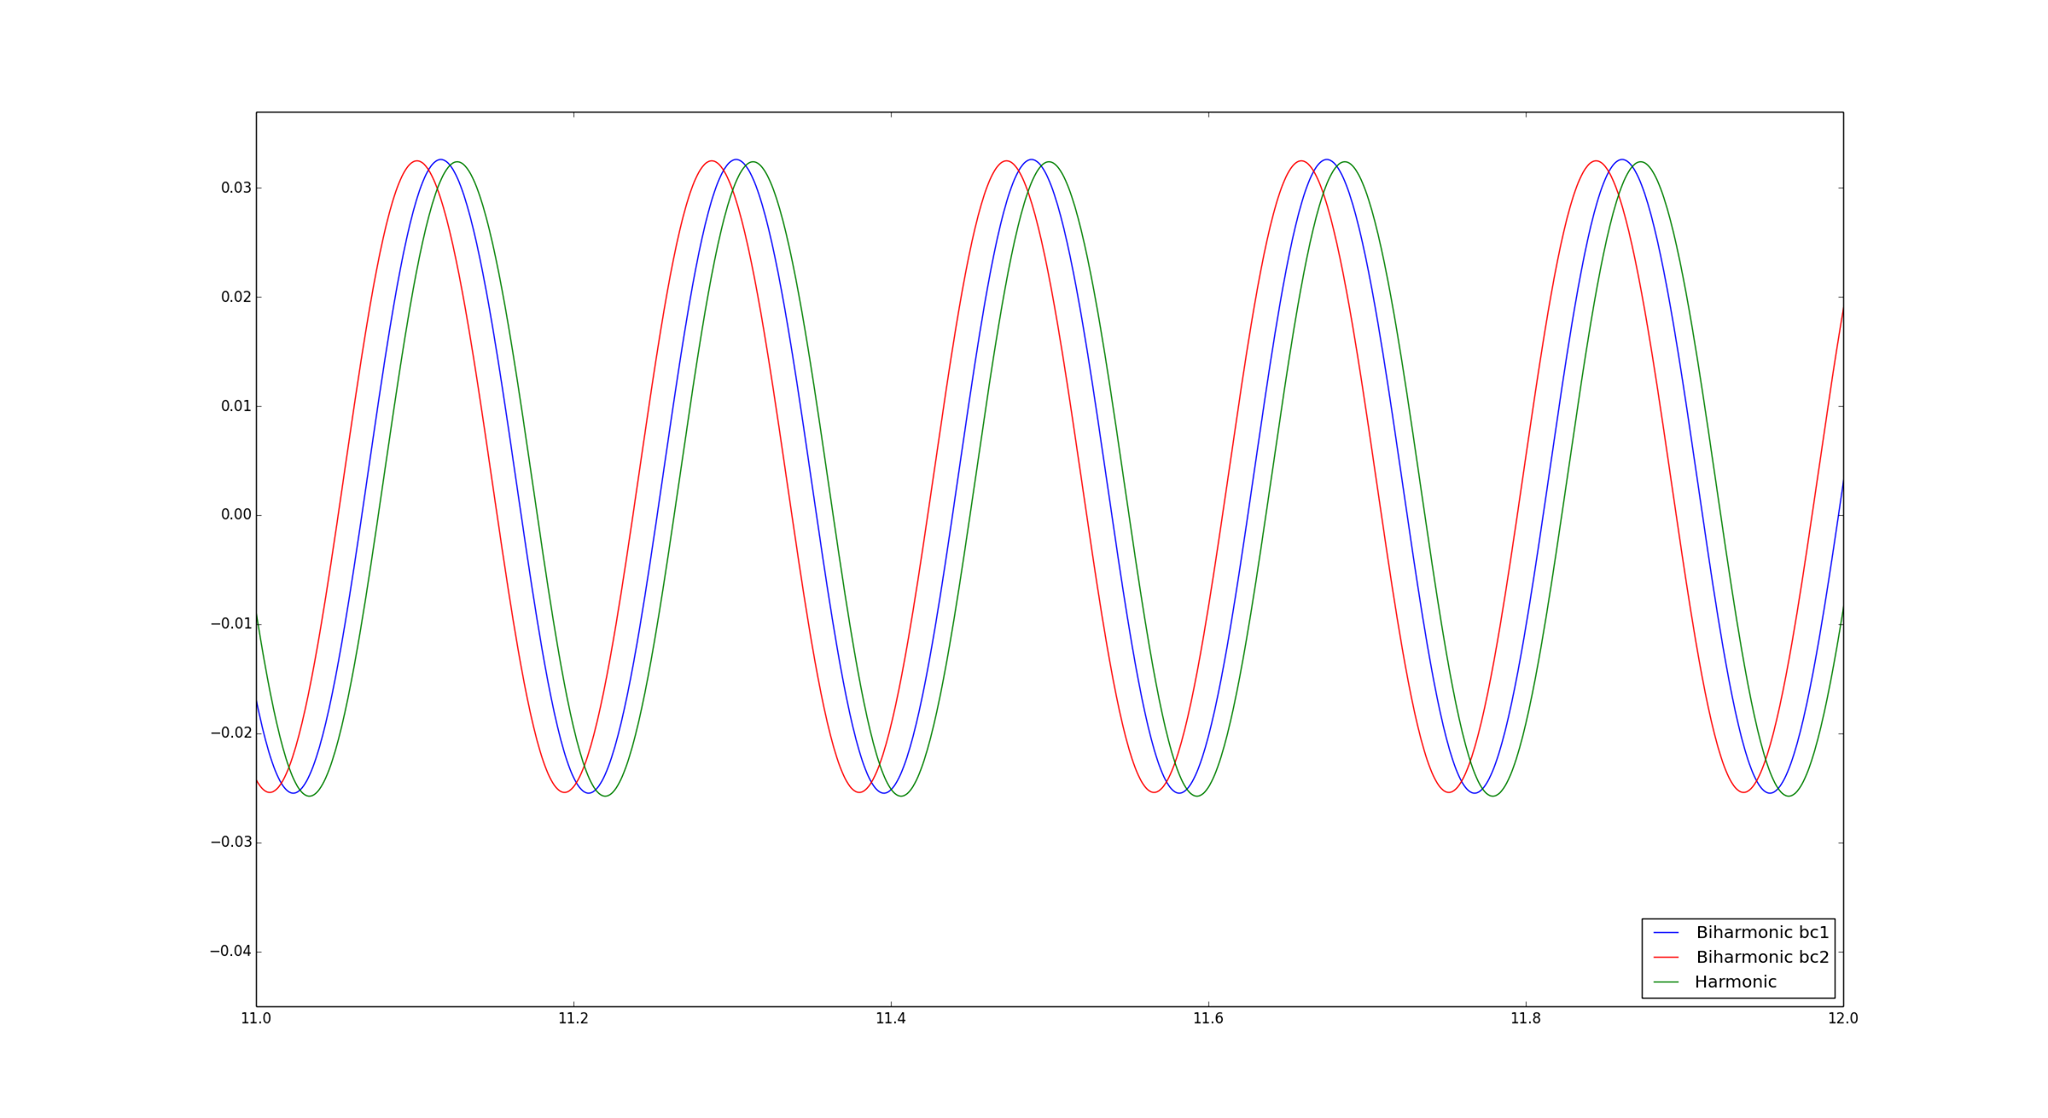
\includegraphics[trim={3cm 3cm 3cm 3cm},scale=0.20]{./Mesh_motion_results/FSI3_dt0001_dis_y.png} 
    \caption{Displacement in x direction for FSI3 with different lifting operators: Harmonic, Biharmonic bc1 and bc2. $\Delta t = 0.001$}
\end{figure}
\begin{figure}[]
    \label{FSI33}
    \centering
    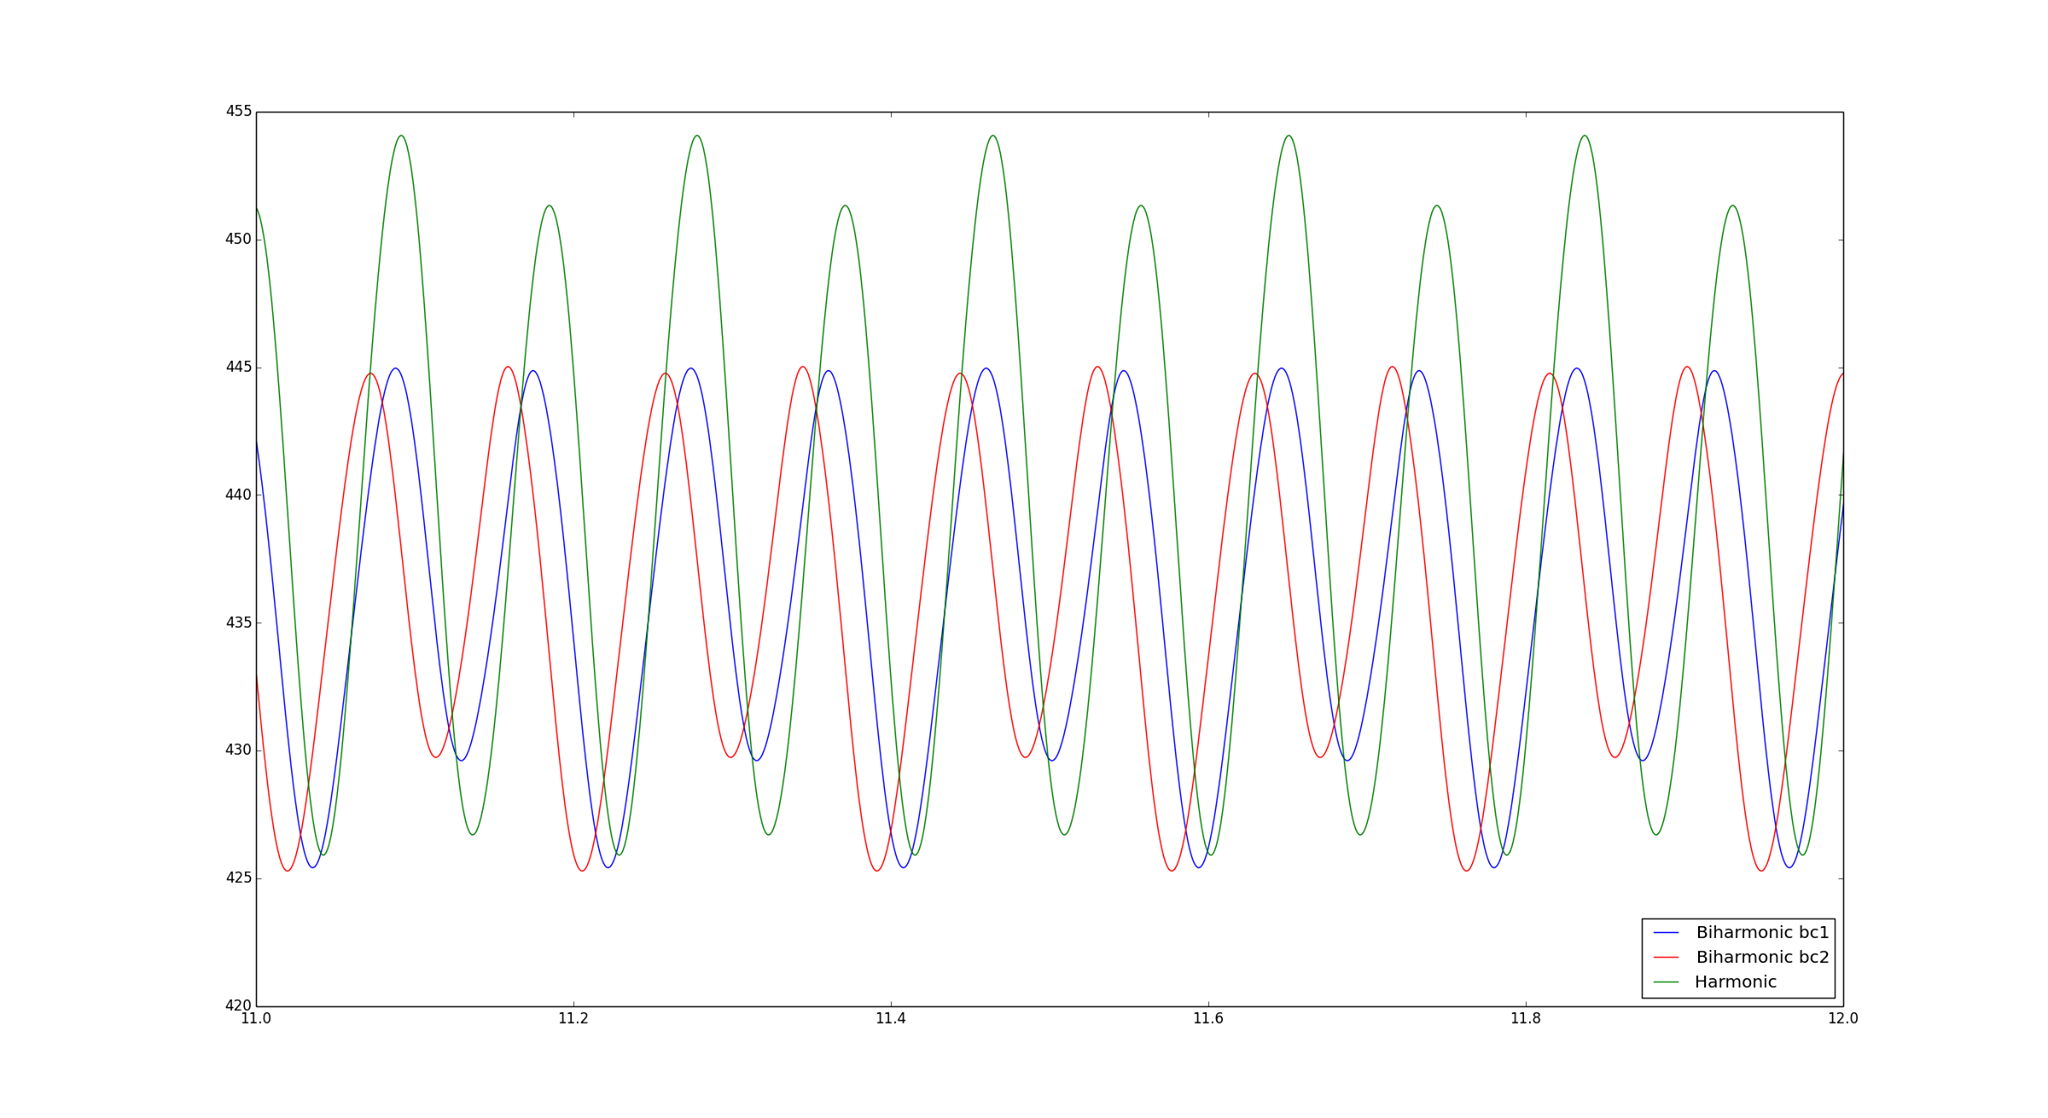
\includegraphics[trim={3cm 3cm 3cm 3cm},scale=0.20]{./Mesh_motion_results/FSI3_dt0001_Drag.png} 
    \caption{Drag results for FSI3 with different lifting operators: Harmonic, Biharmonic bc1 and bc2. $\Delta t = 0.001$}
\end{figure}
\begin{figure}[]
    \label{FSI34}
    \centering
    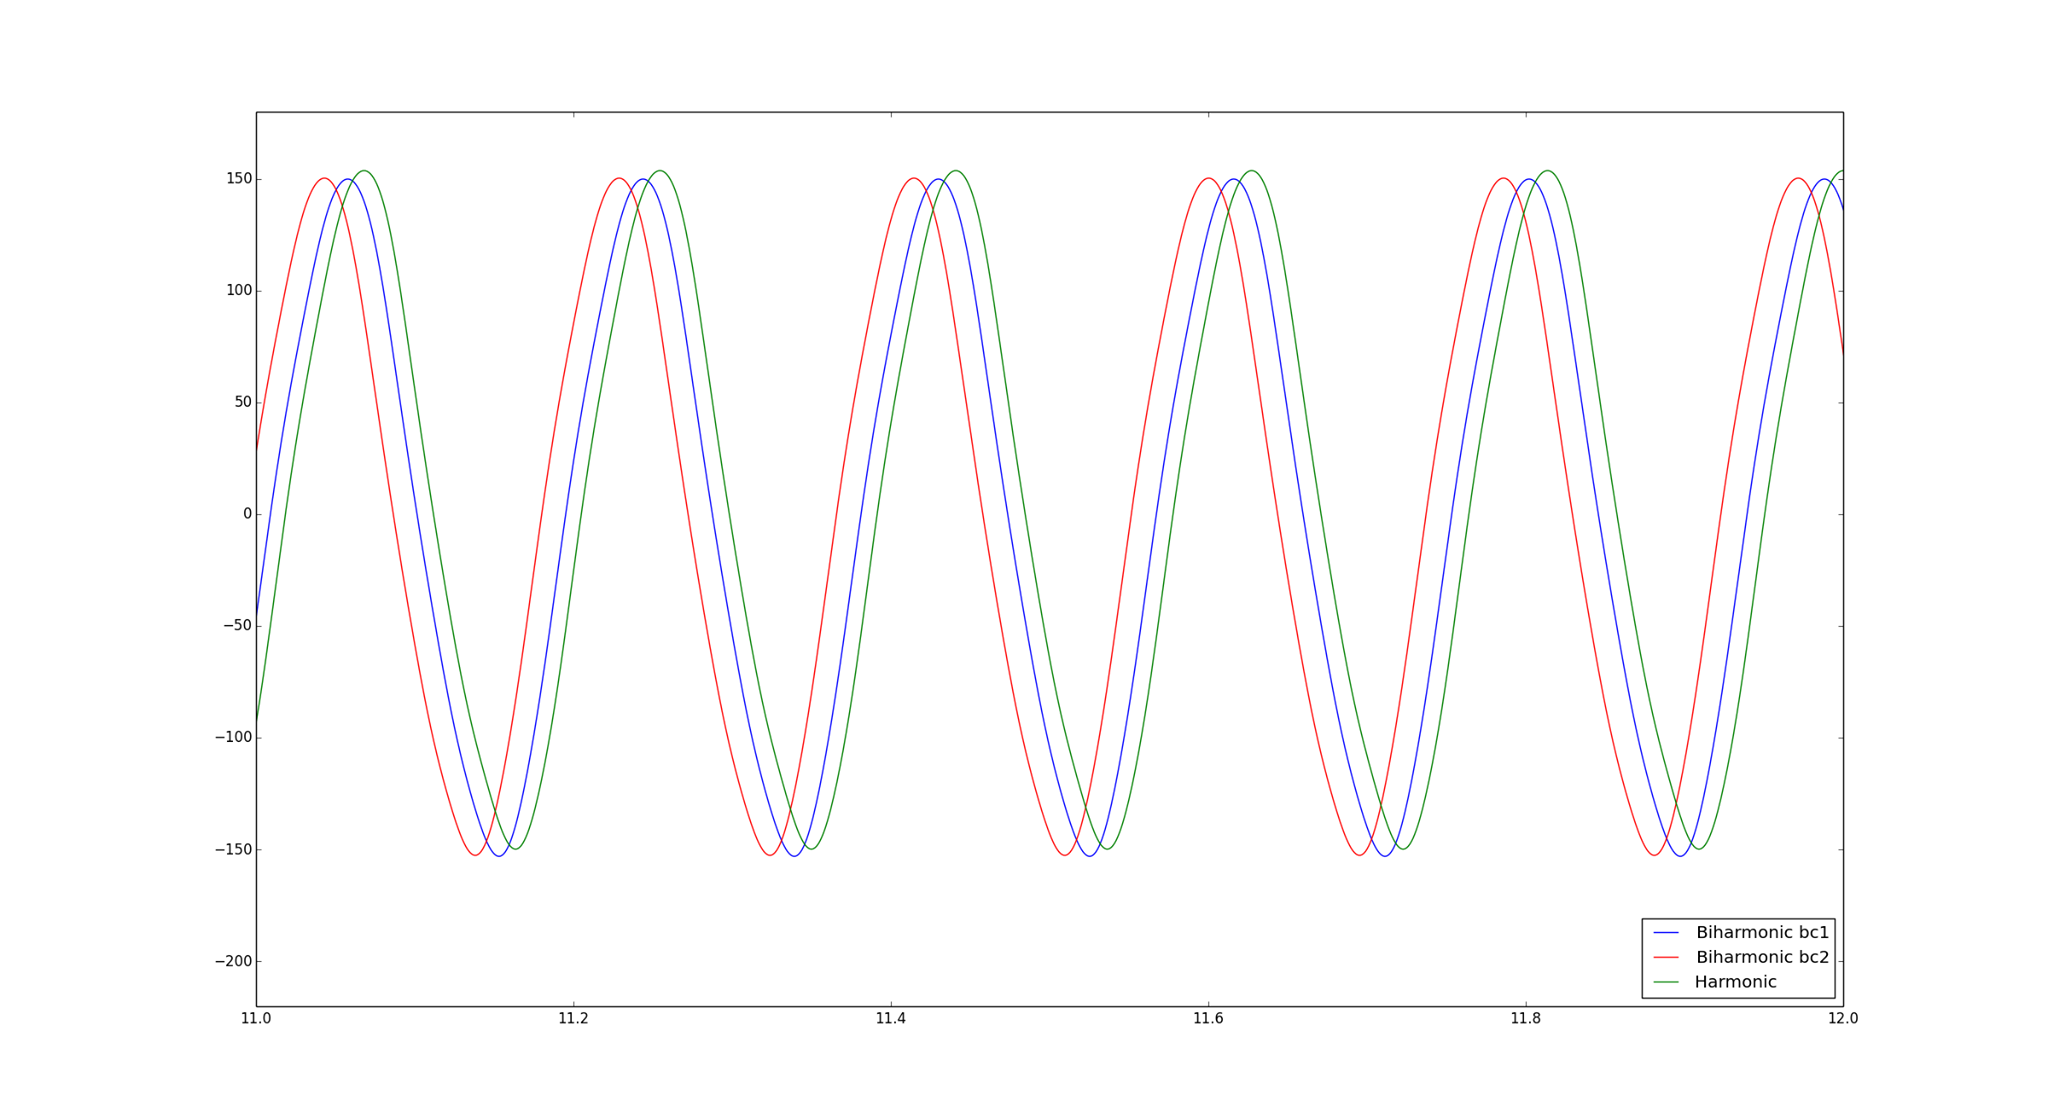
\includegraphics[trim={3cm 3cm 3cm 3cm},scale=0.20]{./Mesh_motion_results/FSI3_dt0001_Lift.png} 
    \caption{Lift results for FSI3 with different lifting operators: Harmonic, Biharmonic bc1 and bc2. $\Delta t = 0.001$}
\end{figure}



\subsection*{Discussion of comparing different lifting operators}
In the FSI2 case all the different lifting operators show similar trend and it is seemingly not important for the results which lifting operator we use. This indicates that with a clever $\alpha_u$, the harmonic technique can be chosen. This is an advantage since the harmonic techniques is the least computationally costly. Whilst when we increase the inflow speed as in the FSI3 case there is a change in the period of the unsteady solution and the drag actually gives higher values. Indicating the the biharmonic lifting operator may be a wiser choice.

In the FSI3 case there is an observed change in the drag values and the reason could be that the cells integrity are upheld in a different manner for different lifting operators. For the harmonic lifting operator it is reasonable to assume that for larger deformations the cell height on the interface will be smaller than for the biharmonic, hence giving a different value to the integrals when calculating drag. The lift and displacement differences for different lifting operators are similar. It is reasonable to assume that this is because of the normal force applied to the upper and lower sides of the bar, which is originally an effect of asymmetry in the y-direction of the domain, is what induces motion. The displacements are a secondary effect of the instability of the fluid and hence the effects we see in the values of lift are also seen in the displacements.

In short the lifting of the deformations into the fluid domain gives different cell structures which in turn effects the integral of the stress tensors on the interface. This in turns produces different results for problems with larger mesh deformations combined with high fluid velocities. This gives the conclusion that lifting operators are highly problem specific and for cases with large deformations lifting operators should be chosen with care.

It should also be noted that the biharmonic lifting operators are able to compute in parallel with multiple computer cores, while the harmonic with variable $\alpha_u$ is not able to run in parallel. This concludes that even though the harmonic lifting operator is is less computationally costly, computing on multiple cores is faster with the biharmonic lifting operator.
\section{Investigating Numerical Stability for Fluid-Structure Interaction Problems}
The following section will give a brief insight in to the effects of choosing different $\theta$ values in the $\theta-$scheme for different time steps. 
The benchmark tests FSI2 and FSI3, as discussed in the previous section, has been investigated since they are known to be numerical unstable for certain values of $\theta$ and $\Delta t$. Only the effects of Drag are reported as the three other quantities shows similar behavior. 
The impact of different $\theta$ values on energy stability in the solid mechanical benchmark CSM3 is also investigated.
\newpage

Figure \ref{fig:FSI2drag_plots} shows the temporal evolution of drag in a simulation with $\Delta t = 0.01$. In the left panel the results are from simulations with $\theta = 0.5 + \Delta t$, and in the right panel $\theta = 0.5$. Based on the results we can observe that a standard Crank-Nicholson scheme becomes unstable when reaching $\sim$13 s. While the shifted Crank-Nicholson,  $\theta = 0.5 + \Delta t$, is stable throughout the simulation.

\begin{figure}[H] 
  \begin{minipage}[b]{0.6\linewidth}
    \centering
    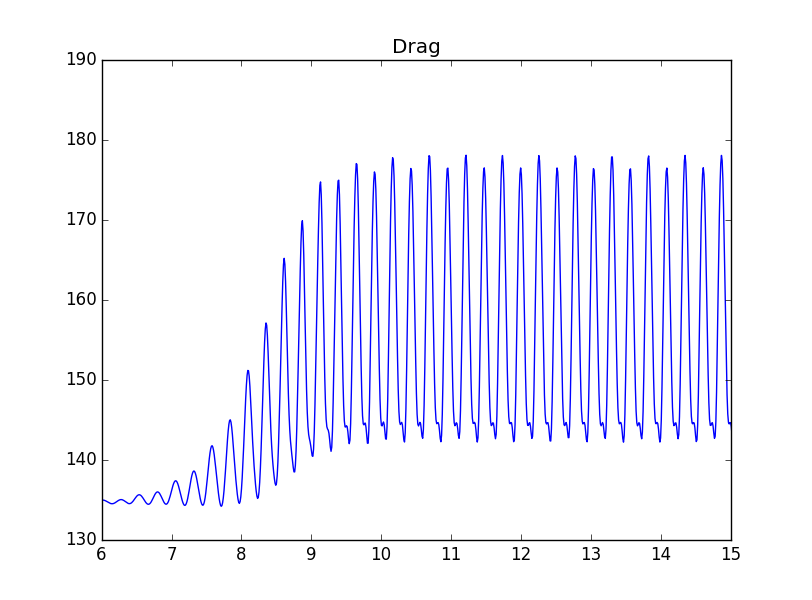
\includegraphics[scale=0.40]{./Temporal_stability/FSI2_001_051_big.png} 
    \caption{Drag vs time with $\theta = 0.50 + \Delta t $} 
    \vspace{4ex}
  \end{minipage}%%
  \begin{minipage}[b]{0.6\linewidth}
    \centering
    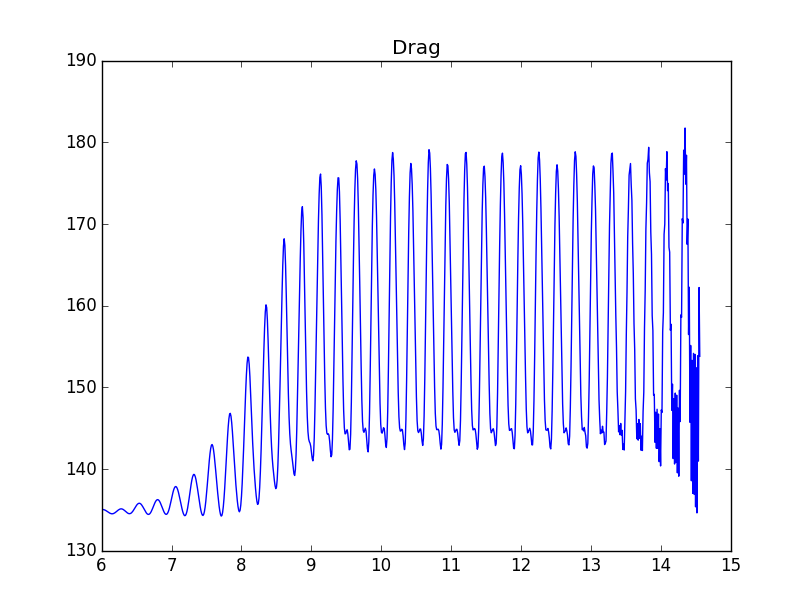
\includegraphics[scale=0.40]{./Temporal_stability/FSI2_001_050_big.png} 
    \caption{Drag vs time with $\theta = 0.50 $} 
    \vspace{4ex}
  \end{minipage} 
  \begin{minipage}[b]{0.6\linewidth}
    \centering
    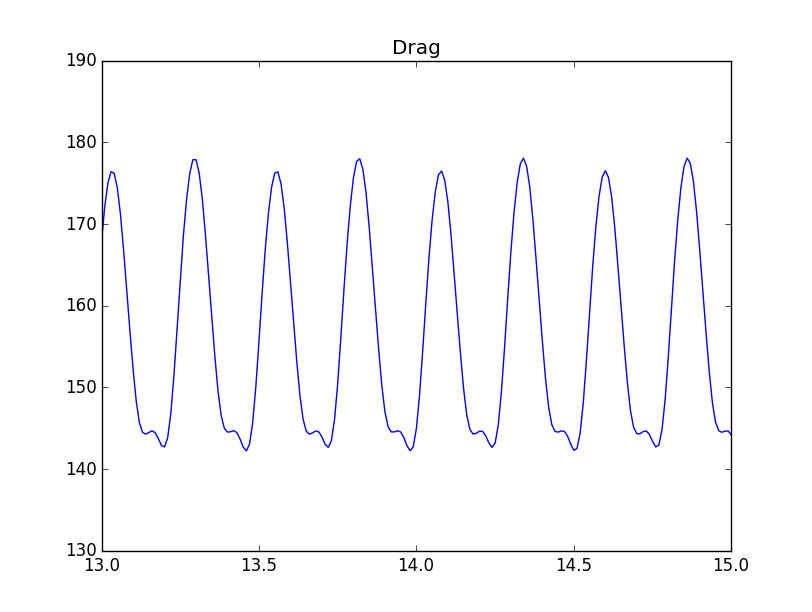
\includegraphics[scale=0.40]{./Temporal_stability/FSI2_001_051_small.png} 
    \caption{Drag vs time with $\theta = 0.50 +\Delta t $} 
    \vspace{4ex}
  \end{minipage}%% 
  \begin{minipage}[b]{0.6\linewidth}
    \centering
    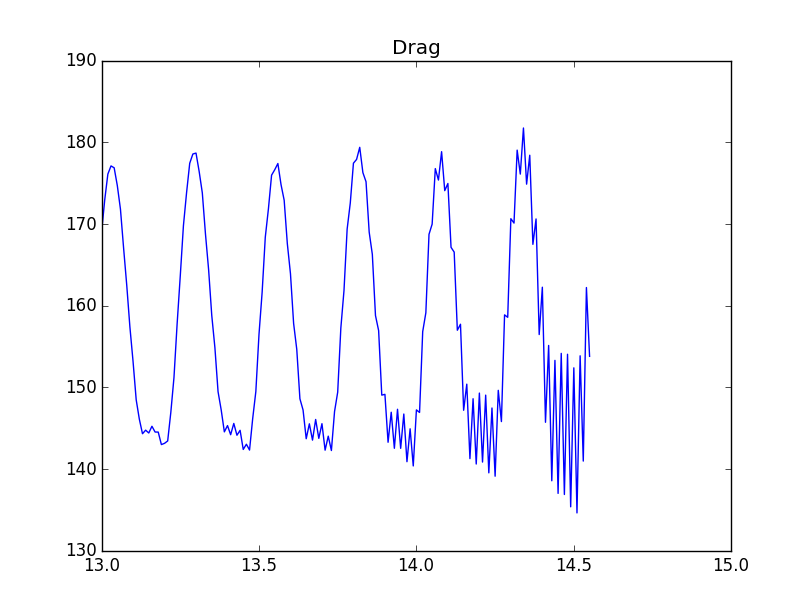
\includegraphics[scale=0.40]{./Temporal_stability/FSI2_001_050_small.png} 
    \caption{Drag vs time with $\theta = 0.50 $} 
    \vspace{4ex}
  \end{minipage} 
\caption {Drag for FSI2 with $\Delta t = 0.01$ with different values for $\theta$}
\label{fig:FSI2drag_plots} 
\end{figure}

Figures \ref{fig: FSI3_long_short} show drag for FSI3 simulation with $\Delta t = 0.001$ and $\theta = 0.5$, showing long term stability for the normal Crank-Nicholson scheme.

\begin{figure}[H]
\begin{tabular}{ll}
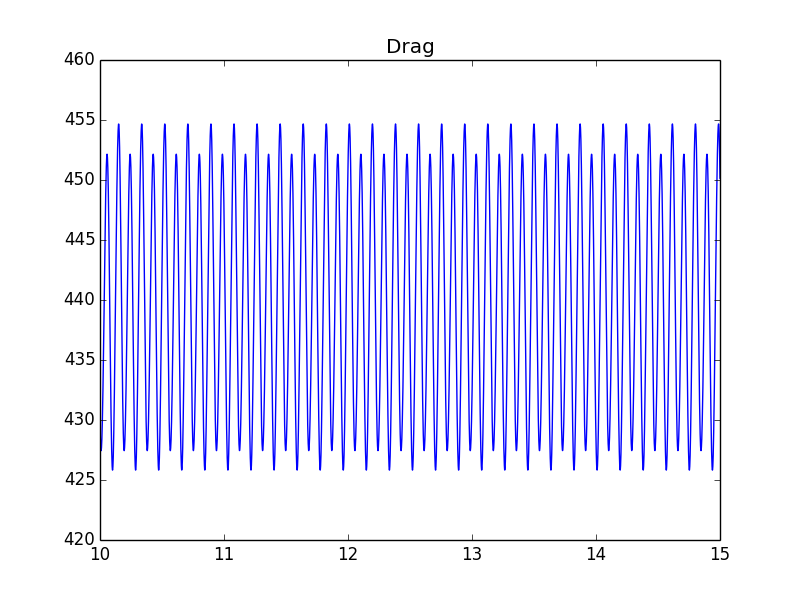
\includegraphics[scale=0.4]{./Temporal_stability/FSI3_0001_050_big.png}
&
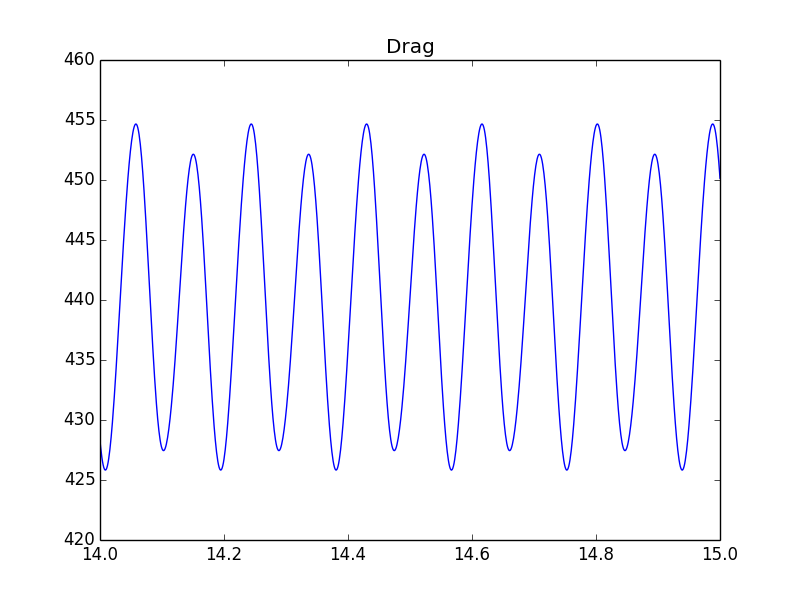
\includegraphics[scale=0.4]{./Temporal_stability/FSI3_0001_050_small.png}
\end{tabular}
\caption{FSI3 drag vs time plot for 10-15 seconds and 14-15 seconds, with $\Delta t = 0.001$ and $\theta =0.5$ showing long term numerical stability}
\label{fig: FSI3_long_short}
\end{figure}

For the CSM3 case only the solid bar is computed, and with an applied force g and no friction, the bar should move down and back up infinitely, for a correct solution.

Figure \ref{fig:CSM3_dis_plots} shows plots of the displacements in x and y directions for $\theta = 0.5$ and $1$. With the implicit scheme ($\theta=1$) the bar moves to a steady state solution. This means energy has not been preserved and the energy dissipates. While in the Crank-Nicholson scheme ($\theta = 0.5$), the bar moves down and back up. This indicates that the Crank-Nicholson scheme is energy preserving.

\begin{figure}[H] 
  \begin{minipage}[b]{0.6\linewidth}
    \centering
    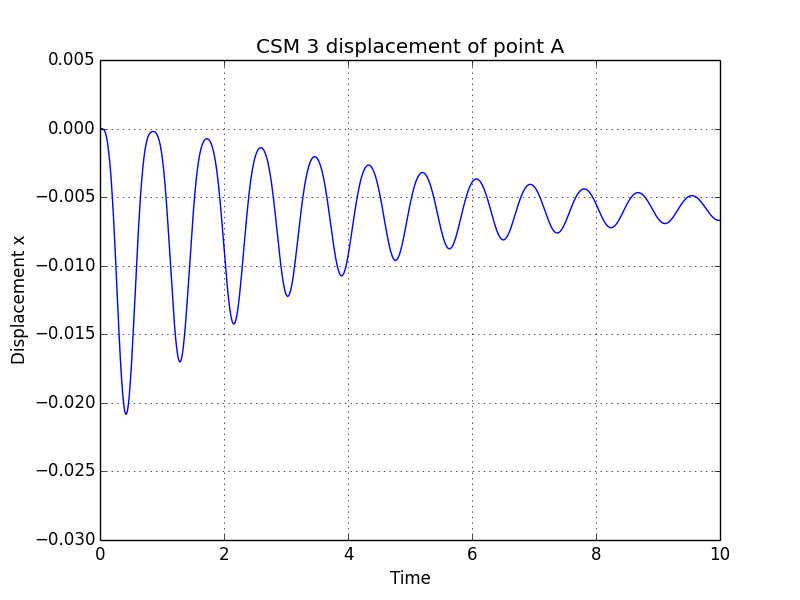
\includegraphics[scale=0.40]{./Temporal_stability/CSM3_implicit.png} 
    \caption{$\theta = 1 $} 
    \vspace{4ex}
  \end{minipage}%%
  \begin{minipage}[b]{0.6\linewidth}
    \centering
    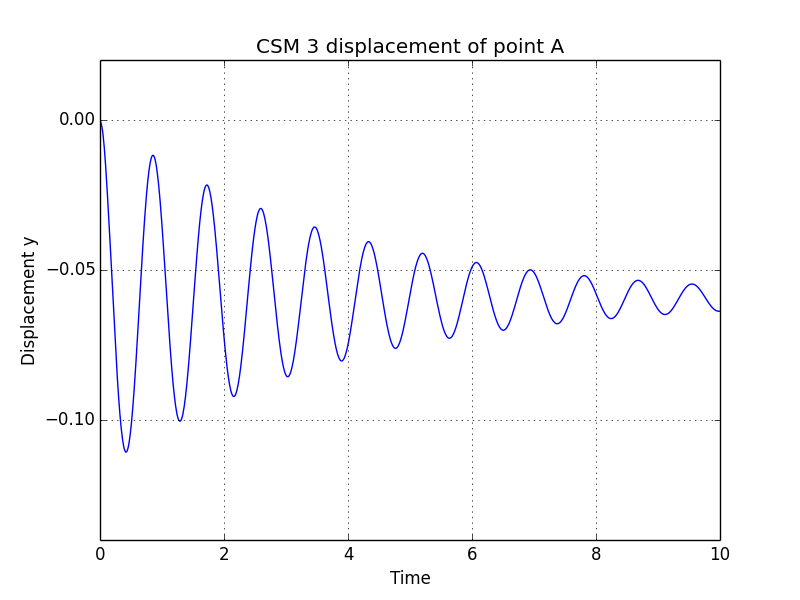
\includegraphics[scale=0.40]{./Temporal_stability/CSM3_implicit_y.png} 
    \caption{$\theta = 1 $} 
    \vspace{4ex}
  \end{minipage} 
  \begin{minipage}[b]{0.6\linewidth}
    \centering
    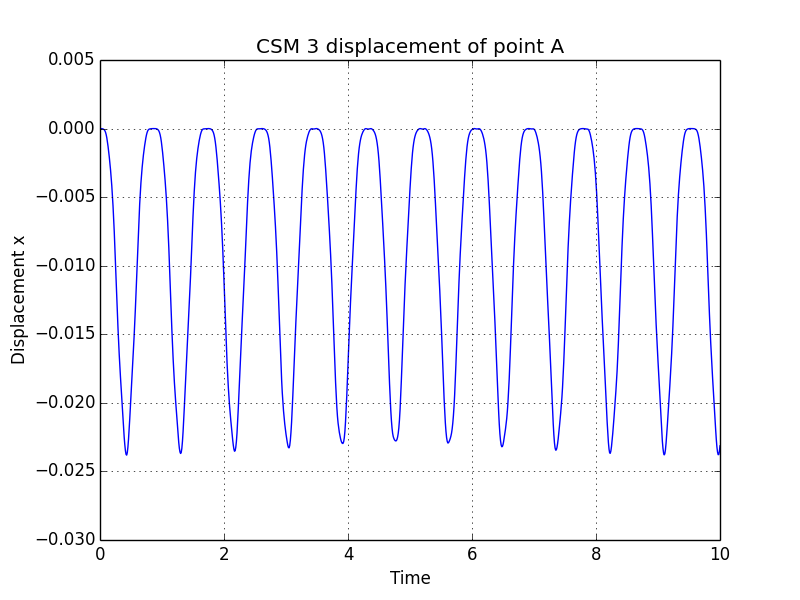
\includegraphics[scale=0.40]{./Temporal_stability/CSM3_Crank.png} 
    \caption{$\theta = 0.5 $} 
    \vspace{4ex}
  \end{minipage}%% 
  \begin{minipage}[b]{0.6\linewidth}
    \centering
    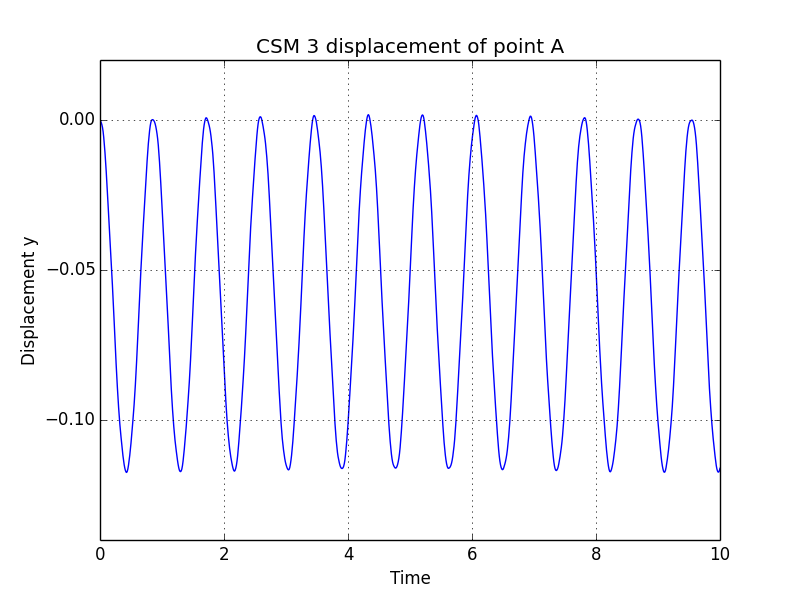
\includegraphics[scale=0.40]{./Temporal_stability/CSM3_Crank_y.png} 
    \caption{$\theta = 0.5 $} 
    \vspace{4ex}
  \end{minipage} 
 \label{fig:CSM3_dis_plots} 
 \caption {CSM3 displacements with $\Delta t = 0.01$ with different values for $\theta$}
\end{figure}


\subsubsection*{Discussion on numerical stability}
The shifted version of the Crank-Nicholson scheme is stable when computing for time step values as low as $\Delta t = 0.01$. However with $\Delta t = 0.001$ the normal Crank-Nicholson scheme ($\theta =0.5$) can be used and is long term stable in the period investigated here. It might be that after 100 s, that the flow would become unstable. However, a rigorous investigation of long-term stability is out of the scope of this thesis. 
It has also been reported by Wick 2011 \cite{Wick2011} that the Crank-Nicholson, $\theta = 0.5$, scheme is stable throughout the computing time by setting $\Delta t = 0.001$.

In the FSI2 case the results for the finest mesh showed, in previous chapter, similar results for $\Delta t = 0.01$ and $\Delta t = 0.001$, meaning that the shifted version of the Crank-Nicholson scheme can be applied, in certain cases, with $\Delta t = 0.01$ greatly reducing computational runtime.

The CSM3 test shows that choosing $\theta = 0.5$ is crucial for preserving energy when computing solid problems. The same property will also be present in a FSI simulation, therefore it is crucial that an energy preserving scheme is applied, otherwise one does not have any control over the artificial numerical dissipation.










